\chapter{Results}

The analysis produced quantitative and visual outputs that describe the spatial distribution, curvature characteristics, and orientation alignment of sweat duct points across the internal fingerprint surface.
\begin{figure}[h!]
    \centering
    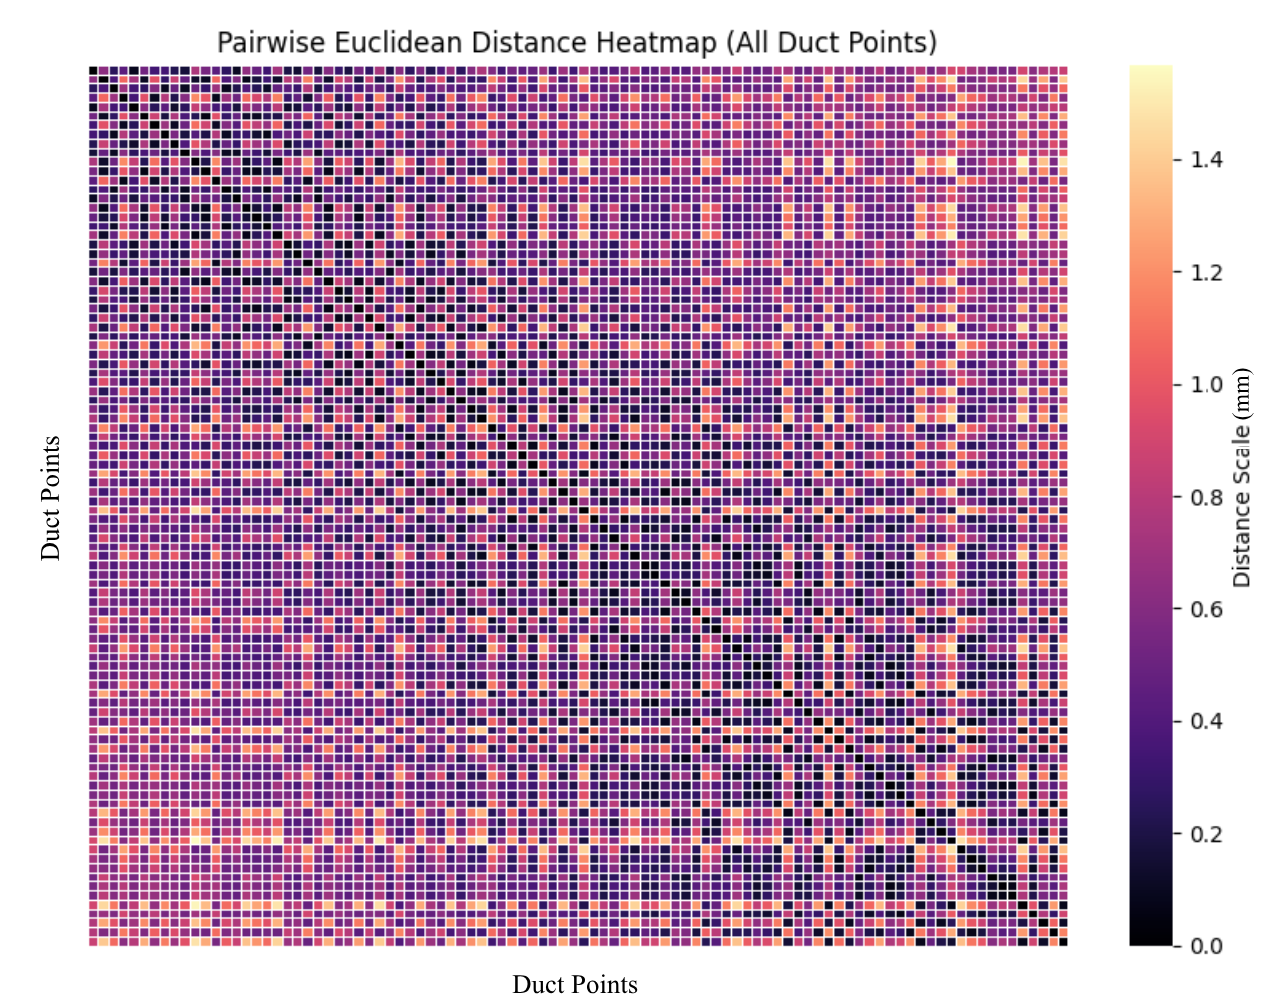
\includegraphics[width=0.9\textwidth]{images/pairwise-heatmap.png}
    \caption{Pairwise heatmap of all sweat duct points on the internal fingerprint surface.}
    \label{fig:pairwise_heatmap}
\end{figure}

Figure~\ref{fig:pairwise_heatmap} shows the pairwise Euclidean distance heatmap for all identified sweat duct points. Each axis represents a duct point index, and colors indicate the Euclidean distance between points. Distances are scaled from $0.0$ to approximately $1.5$ mm. Darker regions correspond to shorter distances, while lighter regions indicate greater separation. Repeating patterns of high- and low-distance values appear across the heatmap. The mean nearest-neighbor distance was $0.1259$ mm (SD = $0.0444$ mm).
\begin{figure}[h!]
    \centering
    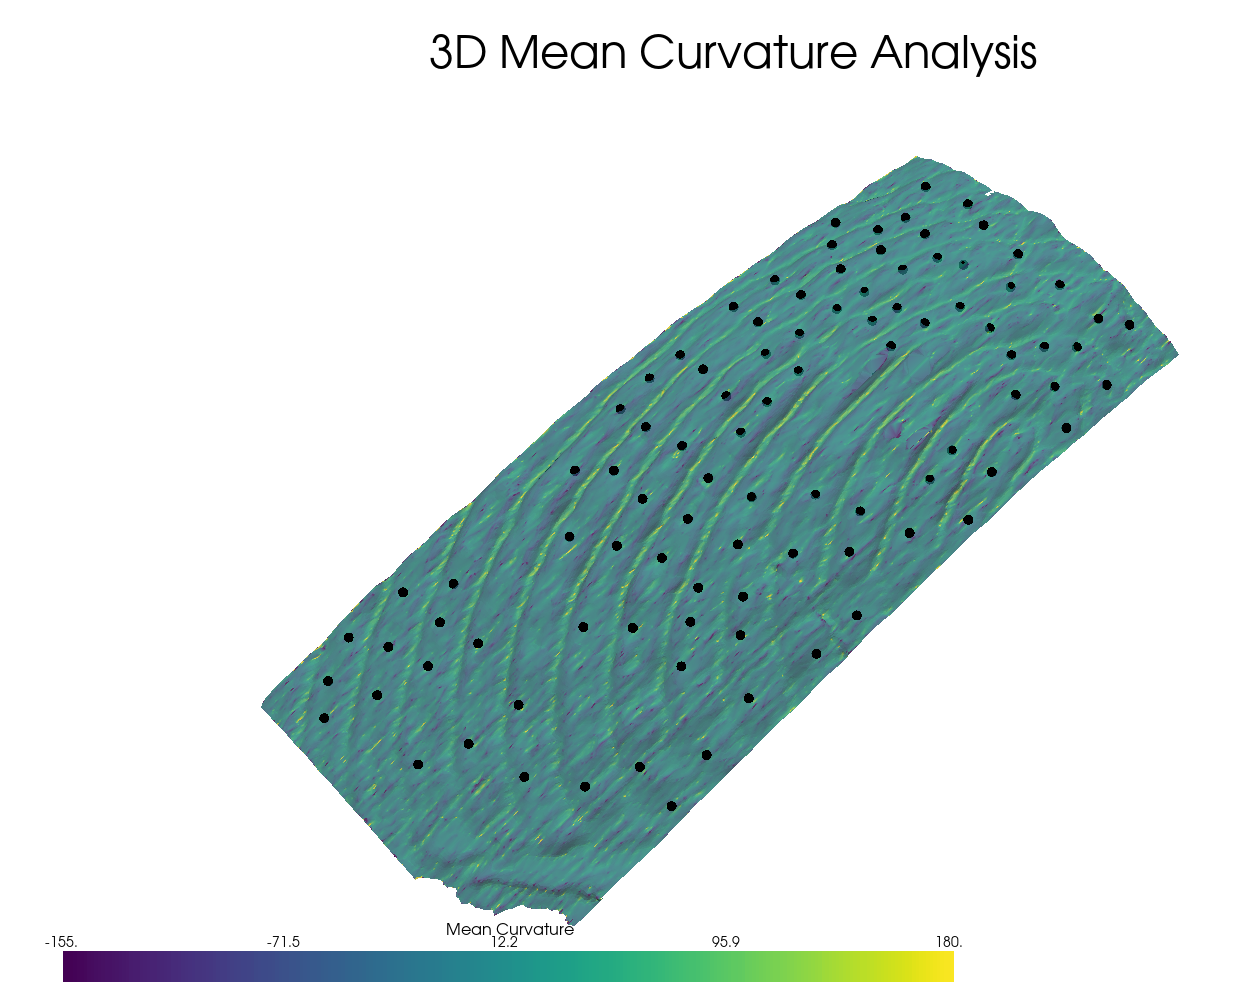
\includegraphics[width=0.9\textwidth]{images/3D_Mean_Curvature_plot.png}
    \caption{3D visualization of mean curvature values on the internal fingerprint surface.}
    \label{fig:curvature_visualization}
\end{figure}

Figure~\ref{fig:curvature_visualization} presents the results of the 3D mean curvature analysis mapped onto the internal fingerprint mesh. The curvature scale ranges from $-155.0$ mm$^{-1}$ to $180.0$ mm$^{-1}$, with cooler colors (purple to blue) representing negative curvature values, warmer colors (green to yellow) representing positive curvature values, and neutral green shades indicating near-zero curvature. Black markers indicate the positions of the sweat duct points used in the analysis. The average mean curvature measured across all sweat duct points and their nearest neighbors was $5.6783$ mm$^{-1}$ (SD = $51.9530$ mm$^{-1}$). A one-sample t-test against a null hypothesis of zero curvature produced a t-statistic of $3.2108$ and a p-value of $1.3726 \times 10^{-3}$. The null hypothesis that curvature equals zero was rejected.
\begin{figure}[h!]
    \centering
    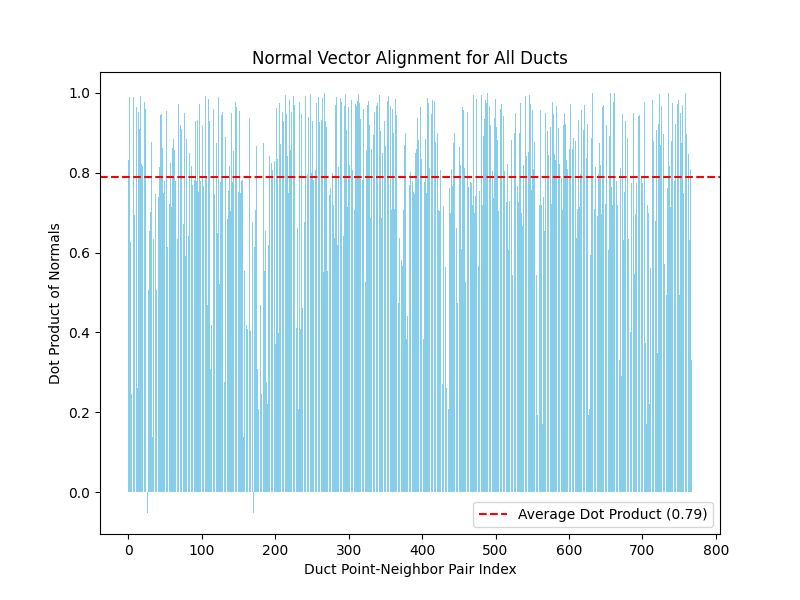
\includegraphics[width=0.9\textwidth]{images/normal_dot_product.png}
    \caption{Distribution of normal vector dot products for sweat duct points and their nearest neighbors.}
    \label{fig:normal_vector_dot_product}
\end{figure}

Figure~\ref{fig:normal_vector_dot_product} shows the distribution of dot product values between the normal vectors of sweat duct points and those of their neighbors. Each bar corresponds to a single point-neighbor pair, with the vertical axis representing the dot product value and the horizontal axis indexing all such pairs. The dashed horizontal red line marks the mean dot product value of $0.7891$. The average dot product of normal vectors was $0.7891$ (SD = $0.1995$). A one-sample t-test comparing the observed mean to a value of perfect alignment ($1.0$) produced a t-statistic of $-29.2802$ and a p-value of $4.2014 \times 10^{-127}$. The null hypothesis of perfect alignment was rejected.
\subsection{Subset Analysis}

A subset of the dataset ($N = 10$) was also analyzed. The mean nearest-neighbor distance was $0.1696$ mm (SD = $0.0679$ mm). The average mean curvature was $4.7877$ mm$^{-1}$ (SD = $31.4448$ mm$^{-1}$), with a t-statistic of $1.5073$ and a p-value of $1.3496 \times 10^{-1}$. The null hypothesis that curvature equals zero was not rejected. The average dot product of normal vectors was $0.8553$ (SD = $0.1458$), with a t-statistic of $-9.2552$ and a p-value of $1.3478 \times 10^{-14}$. The null hypothesis of perfect alignment was rejected.